\chapter{监测设计含义与数值模拟}
\label{chap:design}

第三章得到的方差结构可以回答三个监测设计问题：总报告量固定时期数与单期规模如何取舍；考虑每期固定成本后单期规模应取多大；规模较小时如何可靠地判断疫情是否在增长。前两个问题属于目标Ⅱ，第三个问题属于目标Ⅰ，两类问题对规模的需求相差一个数量级。第~\ref{sec:design-budget}~节至第~\ref{sec:design-test}~节在 H1--H4 下依次讨论这三个问题。第~\ref{sec:design-renewal}~节放宽 H4，用带环境波动的更新过程考察单代结论在时间序列中的适用程度，为第五章的实证设定提供依据。

\section{多期预算分配}
\label{sec:design-budget}

\subsection{期数与单期规模的取舍}

设共观测 $T$ 期，每期预计报告 $m$ 例，总量 $B=Tm$ 固定。用各期估计的平均值 $T^{-1}\sum_t\widehat R_t$ 估计 $\Rbar$。这对应一个常见的监测选择：在一个流行季内，是少数几次大规模调查，还是多次小规模调查。

\begin{proposition}[多期分配]
\label{prop:allocation}
在 H1--H4 下，若各期 $R_t$ 相互独立，则
\begin{equation}
  \frac{1}{T^2}\Var\Bigl(\sum_{t=1}^{T}\widehat R_t\Bigr)=\frac{v_R}{T}+\frac{A}{B}.
  \label{eq:alloc-indep}
\end{equation}
若 $R_t$ 服从系数为 $r\in(0,1)$ 的平稳一阶自回归过程，规模项仍为 $A/B$，环境项变为
\begin{equation}
  \frac{v_R}{T}\cdot\frac{1+r}{1-r}-\frac{2r(1-r^T)\,v_R}{T^2(1-r)^2}.
  \label{eq:alloc-ar}
\end{equation}
两种情形下，方差都随 $T$ 严格递减。
\end{proposition}

推导仍从全方差公式出发，条件变量取全部 $T$ 期的环境 $(R_1,\dots,R_T)$。给定环境，各期的测量误差由各自的传播与报告产生，由 H1 相互独立，条件方差之和为 $\sum_t[R_t/(\rho n)+R_t^2/(kn)]$，取期望后得到 $TA/m$，除以 $T^2$ 即为 $A/(Tm)=A/B$。这一项只依赖总量 $B$，与如何切分无关，也与环境之间是否相关无关，因为环境的相关性只影响各期 $R_t$ 的联合分布，平稳性保证每期的 $\E R_t$ 与 $\E R_t^2$ 不变。条件均值之和为 $\sum_tR_t$，它的方差就是环境项。各期独立时为 $Tv_R$；一阶自回归时滞后 $h$ 的协方差为 $v_Rr^h$，有
\begin{equation}
  \Var\Bigl(\sum_{t=1}^{T}R_t\Bigr)=v_R\Bigl[T+2\sum_{h=1}^{T-1}(T-h)r^h\Bigr],
  \label{eq:ar-sum}
\end{equation}
对几何级数求和即得式~\eqref{eq:alloc-ar}，这是平稳一阶自回归过程部分和方差的精确表达式\citep{hamilton1994time}。

命题~\ref{prop:allocation} 的直觉很简单。总量固定时，规模项 $A/B$ 是固定成本，切成多少期都一样；环境项则取决于看到了多少个独立的环境实现，期数越多，环境偏离被平均得越充分。只看方差，期数越多越好，极端情形是每期只观测极少的病例。现实中期数不能无限增加，第~\ref{sec:design-optimal}~节引入每期固定成本来处理这一点。

\subsection{有效期数近似的偏差}

时间序列分析中常用有效期数 $T_{\mathrm{eff}}=T(1-r)/(1+r)$ 把相关序列折算为独立序列，环境项近似为 $v_R/T_{\mathrm{eff}}$。这一近似只保留了式~\eqref{eq:alloc-ar} 的第一项，第二项为负，所以近似总会高估环境项。高估的相对大小为第二项与精确值之比，第二项与第一项之比为 $2r(1-r^T)/[T(1-r^2)]$，因此近似只在 $T\gg2r/(1-r^2)$ 时可用。$r=0.8$ 时这一门槛约为 4.4，$r=0.5$ 时约为 1.3。

图~\ref{fig:budget}b 画出高估百分比随期数的变化。两条曲线都随 $T$ 单调下降，$r=0.8$ 的曲线始终在 $r=0.5$ 之上，期数很少时高估成倍。$r=0.8$ 时，$T=26$ 高估 20.5\%，$T=10$ 高估 65.8\%，$T=52$ 仍有 9.35\%；$r=0.5$ 时，三者分别为 5.41\%、15.37\% 和 2.63\%。按周观测的流感季通常只有二三十周，周际环境相关又较强，有效期数近似在这一范围内会明显高估环境项，进而低估增加期数的收益。设计计算应直接使用式~\eqref{eq:alloc-ar}。

\subsection{整数约束}

实际切分还受整数约束。每期需要 $n=B/(\rho T)$ 名感染者，因此 $T$ 必须整除 $B/\rho$。例如 $B=30$、$\rho=0.25$ 时，$B/\rho=120$，可行的 $T$ 为 120 的 16 个因数；$\rho=0.7$ 时 $B/\rho$ 非整数，可行集为空，只能放宽总量。整数约束在理论上无关紧要，在报告率较高、总量较小的设计中会直接决定方案是否可行。

\section{成本最优单期规模}
\label{sec:design-optimal}

\subsection{含固定成本的费用模型}

期数不能无限增加，因为每多观测一期都有固定成本，例如启动一轮调查、召集一次会商或维持一个报告周期。设每期固定成本为 $c_0$，每例预计报告病例的边际成本为 $c_1$，总经费为 $\mathcal B$，于是期数 $T=\mathcal B/(c_0+c_1m)$。

\begin{corollary}[成本最优单期规模]
\label{cor:optimal}
在命题~\ref{prop:allocation} 的独立情形下，估计方差为 $f(m)=(c_0+c_1m)(v_R+A/m)/\mathcal B$。当 $c_0>0$ 时，它在下式处取最小值
\begin{equation}
  m^*=\sqrt{\frac{c_0}{c_1}\,\mx},\qquad
  f(m^*)=\frac{(\sqrt{c_0v_R}+\sqrt{c_1A})^2}{\mathcal B}.
  \label{eq:optimal-m}
\end{equation}
若 $\mathcal B<c_0+c_1m^*$，约束 $T\geq1$ 起作用，最优解取 $T=1$；若 $c_0=0$，最优解为 $m\to0$。
\end{corollary}

把 $T=\mathcal B/(c_0+c_1m)$ 代入 $V(m)/T$ 即得 $f(m)$。展开得
\begin{equation}
  \mathcal B\,f(m)=c_0v_R+c_1A+c_1v_R\,m+\frac{c_0A}{m},
  \label{eq:f-expand}
\end{equation}
前两项为常数，后两项一个随 $m$ 线性增加，一个与 $m$ 成反比。令导数 $c_1v_R-c_0A/m^2$ 为零，得 $m^*=\sqrt{c_0A/(c_1v_R)}=\sqrt{(c_0/c_1)\mx}$；二阶导数 $2c_0A/m^3>0$，驻点为最小值。代回后两项相等，均为 $\sqrt{c_0c_1v_RA}$，合并即得 $f(m^*)$。若 $c_0=0$，后一项消失，$f$ 随 $m$ 单调增加，回到命题~\ref{prop:allocation} 的结论，即没有固定成本时，期数越多越好。

式~\eqref{eq:f-expand} 揭示了权衡的两端。$c_1v_Rm$ 对应单期规模过大，经费集中在少数几期，看到的环境实现太少；$c_0A/m$ 对应单期规模过小，期数太多，固定成本挤占了病例经费，每期的测量误差偏大。最优单期规模是成本比 $c_0/c_1$ 与交叉点 $\mx$ 的几何平均。固定成本相对越高，每期越应多收集病例；交叉点越大，即环境越稳定或测量噪声越大，每期也越应多收集病例。最优规模与总经费 $\mathcal B$ 无关，经费增加只改变期数。

\subsection{与两阶段抽样的同构}

推论~\ref{cor:optimal} 与两阶段抽样的费用最优分配是同一个问题\citep{cochran1977sampling}。对照式~\eqref{eq:two-stage} 与式~\eqref{eq:cochran-opt}，期数 $T$ 对应初级单元数，$v_R$ 对应初级单元间方差 $S_b^2$，$A$ 对应单元内方差 $S_w^2$，$c_0$ 与 $c_1$ 分别对应初级单元与次级单元的单位成本 $c_1'$、$c_2'$。两个最优解的形式完全相同，都是费用比与方差比之积的平方根。

同构也提示了差别所在。两阶段抽样中初级单元按设计独立抽取，监测中的各期环境存在时间相关；抽样中单元内样本量由设计者决定，监测中的规模由此前的传播产生。前一个差别在下文的自相关修正中处理，后一个差别对应 H4，在第~\ref{sec:design-renewal}~节讨论。

\subsection{数值示例}

按第五章的情景参数，交叉点 $\mx$ 在 21.3--49.2。$c_0/c_1=10$ 时 $m^*$ 为 14.6--22.2，$c_0/c_1=100$ 时为 46.1--70.1。在第三章的示例参数下（$\mx=53.1$），两种成本比对应的 $m^*$ 分别为 23.0 和 72.9。成本比扩大 10 倍，最优规模只扩大约 3.2 倍，这是平方根关系的直接结果。

连续解需要取整后才能执行。取示例参数，$c_0=100$，$c_1=1$，$\mathcal B=600$，连续解为 $m^*=72.86$，对应方差 $f(m^*)=0.01992$，此时 $T=600/172.86$ 不是整数。表~\ref{tab:integer-alloc} 逐个列出整数 $T$ 下的方案，单期规模由 $m=\mathcal B/T-c_0$ 得到。

\begin{table}[!tbp]
  \centering
  \caption{固定经费下整数期数方案的比较}
  \label{tab:integer-alloc}
  \begin{tabular}{@{}cccc@{}}
    \toprule
    期数 $T$ & 单期规模 $m$ & 估计方差 & 与连续最优之比 \\
    \midrule
    1 & 500 & 0.04425 & 2.22 \\
    2 & 200 & 0.02531 & 1.27 \\
    3 & 100 & 0.02041 & 1.02 \\
    4 & 50 & 0.02062 & 1.04 \\
    5 & 20 & 0.02923 & 1.47 \\
    \bottomrule
  \end{tabular}

  \vspace{4pt}
  {\small 注：$\overline{R}=1.15$，$v_R=0.04$，$k=0.35$，$\rho=0.25$，$c_0=100$，$c_1=1$，$\mathcal{B}=600$；连续最优为 $m^*=72.86$，方差 0.01992。}
\end{table}

最优整数方案是 $T=3$、$m=100$，方差 0.02041，只比连续最优高约 2.5\%；$T=4$、$m=50$ 次之。把经费全部投入一期（$T=1$）的方差是最优方案的两倍多，切成五期（$T=5$）则因固定成本占去大部分经费，每期只剩 20 例，方差也明显偏高。图~\ref{fig:budget}a 画出连续目标函数与五个整数方案。曲线在 $m^*$ 左侧陡峭、右侧平缓：规模不足时方差上升很快，规模偏大时上升较慢。这一不对称来自式~\eqref{eq:f-expand} 中反比项与线性项的形状差异，它意味着在参数不确定时，宁可把单期规模取得略大一些。

\begin{figure}[!tbp]
  \centering
  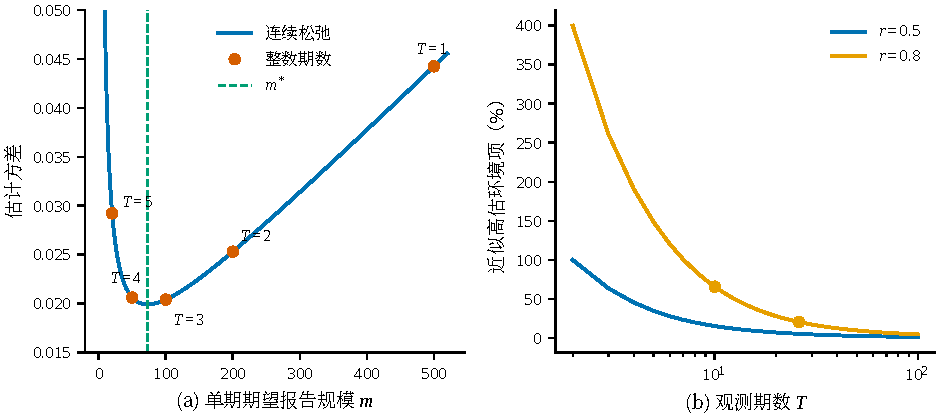
\includegraphics[width=\textwidth]{figures/fig_4_1_budget.pdf}
  \caption{预算分配的两个侧面。（a）固定经费下估计方差随单期规模的变化，$c_0=100$，$c_1=1$，$\mathcal{B}=600$，其余参数取示例值；曲线为连续松弛，圆点为整数期数方案，竖虚线为连续最优 $m^*$。（b）环境服从一阶自回归时，有效期数近似相对精确式高估环境项的百分比随观测期数的变化，圆点标出 $r=0.8$ 时 $T=10$ 与 $T=26$。}
  \label{fig:budget}
\end{figure}

\subsection{自相关修正}

若环境服从一阶自回归，式~\eqref{eq:alloc-ar} 的第一项相当于把环境方差放大为 $v_R(1+r)/(1-r)$，交叉点相应缩小为原来的 $(1-r)/(1+r)$ 倍，$m^*$ 应乘以约 $\sqrt{(1-r)/(1+r)}$。最优方案因而偏向更多、更小的期。这一方向初看有违直觉：相邻各期的环境相似，多观测一期带来的新信息变少，似乎应当减少期数。决定权衡的却是两项的相对大小。环境项被放大后，规模项在总方差中的份额下降，压低环境项的边际价值相对上升，而压低环境项只能靠增加期数。

仍取示例参数与 $c_0/c_1=100$，$r=0.5$ 时数值求得的精确最优与近似值分别为 42.9 和 42.1，$r=0.8$ 时分别为 25.0 和 24.3。近似值比精确值略小，这与有效期数近似高估环境项的方向一致，二者相差不到 1 例，近似在设计中够用。

\section{精确增长检验}
\label{sec:design-test}

\subsection{检验的构造}

监测中最常见的判断是疫情是否在增长，即检验 $H_0\colon R_t\leq1$ 对 $H_1\colon R_t>1$。这是目标Ⅰ层面的问题，误差只来自测量，规模的作用持续存在。

\begin{proposition}[精确增长检验]
\label{prop:test}
在 H1--H3 下，$C_t$ 的分布族关于 $R_t$ 具有单调似然比。令 $c_\alpha$ 为满足 $P_{R_t=1}(C_t\geq c)\leq\alpha$ 的最小整数，检验在 $C_t\geq c_\alpha$ 时拒绝 $H_0$。该检验有以下三条性质。
\begin{enumerate}[label=(\roman*)]
  \item 第一类错误概率在 $R_t\leq1$ 上的上确界在 $R_t=1$ 处取得，实际水平 $\alpha^*\leq\alpha$。
  \item 该检验在水平 $\alpha^*$ 下一致最优；加入随机化的 Karlin--Rubin 检验恰好达到水平 $\alpha$，并在该水平下一致最优。
  \item 在 $R_t=1+\delta$ 处的功效为
  \begin{equation}
    \pi(n,\delta)=1-F_{\NB}\bigl(c_\alpha-1;\ nk,\ k/[k+\rho(1+\delta)]\bigr).
    \label{eq:power}
  \end{equation}
\end{enumerate}
\end{proposition}

单调似然比性质可以直接验证。取 $R_2>R_1$，由式~\eqref{eq:report-dist}，似然比为
\begin{equation}
  \frac{f(c;R_2)}{f(c;R_1)}=\Bigl(\frac{k+\rho R_1}{k+\rho R_2}\Bigr)^{nk}
  \Bigl[\frac{R_2(k+\rho R_1)}{R_1(k+\rho R_2)}\Bigr]^{c},
  \label{eq:mlr}
\end{equation}
方括号内的底数大于 1，因为 $R_2k+\rho R_1R_2>R_1k+\rho R_1R_2$，所以似然比随 $c$ 递增。由 Karlin--Rubin 定理，形如 $\{C_t\ge c\}$ 的拒绝域在它自身的实际水平下一致最优，拒绝概率随 $R_t$ 递增，零假设下的最大第一类错误概率出现在边界 $R_t=1$ 处\citep{karlin1956theory, lehmann2005testing}。功效公式~\eqref{eq:power} 是负二项分布函数在临界值处的直接计算。

这里的“一致最优”需要限定。非随机化检验只能在 $\alpha^*$ 这个离散的水平上一致最优；要在名义水平 $\alpha$ 上最优，需要在 $C_t=c_\alpha-1$ 时以一定概率随机拒绝，这在监测实践中难以接受。命题~\ref{prop:test} 还依赖 $k$ 已知；若 $k$ 用数据估计，水平不再有精确保证。$k$ 设得过大会低估方差，临界值偏低，实际水平随之偏高；设得过小则检验偏保守。

\subsection{Wald 检验的水平失真}

实际工作中常用正态近似的 Wald 检验，即把 $(\widehat R_t-1)/\sqrt{V_0}$ 与正态分位数比较，其中 $V_0=1/(\rho n)+1/(kn)$ 是 $R_t=1$ 时的方差。该检验的实际水平同样可以用负二项分布函数精确算出，不需要模拟。

图~\ref{fig:test}a 给出名义水平为 5\% 时两种检验的实际水平。彩色点为 Wald 检验，三种颜色对应三个 $k$ 值；灰色点为精确检验。Wald 检验在小规模时系统性地超过名义水平，点群整体落在 5\% 虚线之上，并随规模增大逐渐向虚线靠拢。$k=0.1$、$m=5$ 时实际水平为 7.81\%；在 $m<40$ 的范围内，$k=0.1$、0.35 和 1 的最大实际水平分别为 8.03\%、8.75\% 和 10.40\%。精确检验的点全部在虚线以下，整个网格上的最大水平为 0.05000，没有超出名义水平。两种检验的点都呈锯齿状排列，这是离散分布下临界值逐格跳动的结果。

Wald 检验偏离的原因是负二项分布在小规模时右偏明显。右偏分布的上尾比正态分布厚，用正态分位数作临界值会把过多的零假设样本判为增长。这与 Brown 等在二项比例区间中发现的问题同类\citep{brown2001interval}，负二项计数的偏度还要更大。对监测实践而言，若用 Wald 检验在小辖区每周判断增长，误报的频率会比预设高出一半到一倍。

\begin{figure}[!tbp]
  \centering
  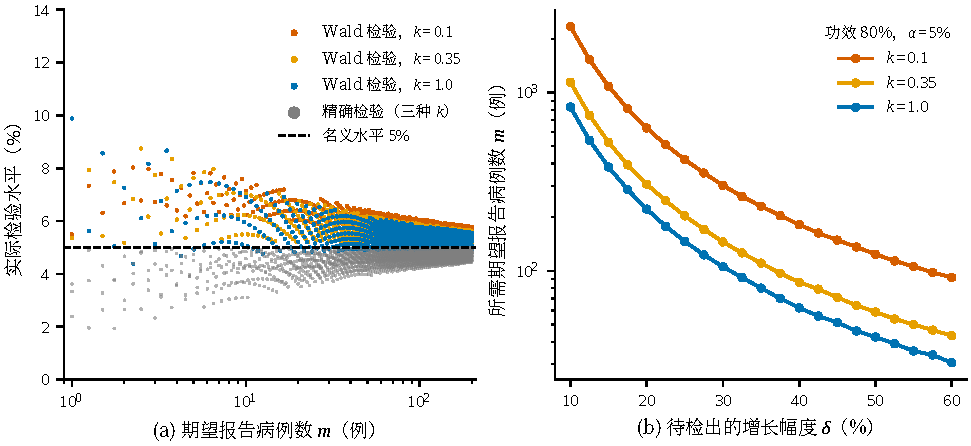
\includegraphics[width=\textwidth]{figures/fig_4_3_growth_test.pdf}
  \caption{增长检验的实际水平与所需规模，$\rho=0.25$，名义水平 5\%，全部由负二项分布函数精确计算。（a）Wald 检验（按 $k$ 着色）与精确检验（灰色）的实际水平随期望报告规模的变化；（b）达到并保持 80\% 功效所需的期望报告规模与待检出增长幅度 $\delta$ 的关系。}
  \label{fig:test}
\end{figure}

\subsection{功效的锯齿与所需规模}

功效随 $n$ 的变化不是单调的。$c_\alpha$ 只能取整数，每当它跳升一格，实际水平骤降，功效也随之短暂下降。以 $k=0.35$、$\delta=0.3$ 为例，$n$ 从 400 增加到 699 的过程中，功效下降了 82 次。因此只报告“首次达到 80\% 功效的规模”并不够，略大一点的规模可能又跌回 80\% 以下；更稳妥的指标是“此后始终保持 80\% 以上的最小规模”。表~\ref{tab:power-n} 同时列出两者。

\begin{table}[!tbp]
  \centering
  \caption{增长检验达到 80\% 功效所需的感染者人数}
  \label{tab:power-n}
  \begin{tabular}{@{}cccc@{}}
    \toprule
    离散参数 $k$ & 增长幅度 $\delta$ & 首次达到 & 此后保持 \\
    \midrule
    0.35 & 0.15 & 2071 & 2107 \\
    0.35 & 0.30 & 568 & 581 \\
    0.35 & 0.50 & 229 & 235 \\
    1 & 0.25 & 568 & 585 \\
    0.1 & 0.25 & 1660 & 1684 \\
    \bottomrule
  \end{tabular}

  \vspace{4pt}
  {\small 注：$\rho=0.25$，名义水平 5\%，单侧检验；表中为上一代感染者人数 $n$，预计报告规模为 $m=\rho n$。}
\end{table}

表~\ref{tab:power-n} 有三点规律。增长幅度越小，所需规模越大，$\delta$ 从 0.5 降到 0.15，所需人数扩大约 9 倍，大致与 $\delta^{-2}$ 成比例，这是正态近似下功效计算的一般规律。离散参数越小，所需规模越大，$\delta=0.25$ 时 $k=0.1$ 所需人数约为 $k=1$ 的 2.9 倍，超传播让每一个病例携带的信息变少。首次达到与此后保持之间的差距为 6 至 36 人，相对差距在 1\% 至 3\% 之间，绝对值不大，但在规模本已较大时，按首次达到的数字设计会有一段规模区间功效不足。图~\ref{fig:test}b 以预计报告规模为纵轴画出保持 80\% 功效所需的规模，三条曲线随 $\delta$ 增大而下降，$k$ 越小曲线越高，规律与表~\ref{tab:power-n} 一致。

这些数字与第三章的交叉点形成对照。$k=0.35$ 时，要稳定检出 15\% 的增长，每期需要约 2107 名感染者，即 $m\approx527$ 例预计报告，是示例交叉点的十倍左右。对目标Ⅱ而言，规模过了 $\mx$ 收益就明显变小；对判断当期增长这类目标Ⅰ问题，规模的价值要大得多。同一套监测数据服务于不同目标时，规模是否“够用”的答案可以完全不同。

\section{时间序列中的规模效应}
\label{sec:design-renewal}

\subsection{随机分母问题}

前几节假定上一代感染者人数 $n$ 已知。真实监测序列不满足这一点。下一周的新感染由此前几周的感染共同产生，感染压力可写为 $\Lambda_{t+1}=\sum_{s\geq1}w_sI_{t+1-s}$，其中 $w_s$ 是世代间隔分布。漏报使 $I_1,\dots,I_t$ 无法完全观测，所以下一周的感染压力 $\Lambda_{t+1}$ 也是随机的。实际能用的只是报告数的加权和
\begin{equation}
  D_t=\sum_{s\geq1}w_sC_{t+1-s},
  \label{eq:dt}
\end{equation}
并以 $G_t=C_{t+1}/D_t$ 作为增长统计量。$D_t$ 在这里扮演了 $m=\rho n$ 的角色，但它本身含有报告噪声，是一个随机分母。

预测误差取决于可用的信息集。记 $\mathcal F_t$ 为截至第 $t$ 周的全部报告，$m=\rho\,\E(\Lambda_{t+1}\mid\mathcal F_t)$。

\begin{remark}
\label{rem:information}
设给定 $\Lambda_{t+1}$ 与 $R_{t+1}$ 时，$C_{t+1}$ 服从式~\eqref{eq:report-dist} 中以 $\Lambda_{t+1}$ 代替 $n$ 的负二项分布，且在 $\mathcal F_t$ 条件下 $\Lambda_{t+1}$ 与 $R_{t+1}$ 独立。两次使用全方差公式，可得
\begin{equation}
  \frac{\Var(C_{t+1}\mid\mathcal F_t)}{[\rho\,\E(\Lambda_{t+1}\mid\mathcal F_t)]^2}
  =v_R+\frac{A}{m}+\CV^2(\Lambda_{t+1}\mid\mathcal F_t)\,(\Rbar^2+v_R).
  \label{eq:info-decomp}
\end{equation}
当 $\Lambda_{t+1}$ 完全已知时，变异系数项为零，式~\eqref{eq:info-decomp} 退化为命题~\ref{prop:average}。
\end{remark}

注~\ref{rem:information} 的推导分两层。第一层条件于 $(\Lambda_{t+1},R_{t+1})$，条件均值为 $\rho\Lambda_{t+1}R_{t+1}$，条件方差的期望按命题~\ref{prop:average} 的方式处理，得到规模项。第二层计算条件均值 $\rho\Lambda_{t+1}R_{t+1}$ 在 $\mathcal F_t$ 下的方差，利用 $\Lambda_{t+1}$ 与 $R_{t+1}$ 条件独立，乘积的方差拆为 $\E(\Lambda^2)\E(R^2)-[\E\Lambda\,\E R]^2$，除以 $(\rho\E\Lambda)^2$ 后得到 $v_R$ 与 $\CV^2(\Lambda)(\Rbar^2+v_R)$ 两项。多出的一项来自感染压力的不确定性，它与规模无关。漏报使感染压力无法由报告精确还原，因此这一项在实际序列中一般不为零。

\subsection{误差指标的两种读法}

第五章使用的误差指标有两种读法。用 $\Rbar D_t$ 预测 $C_{t+1}$ 的相对误差，与用 $G_t$ 估计 $\Rbar$ 的相对误差恒等：
\begin{equation}
  \frac{(C_{t+1}-\Rbar D_t)^2}{(\Rbar D_t)^2}=\frac{(G_t-\Rbar)^2}{\Rbar^2}.
  \label{eq:identity}
\end{equation}
左端是预测问题，右端是估计问题，二者在数值上相同。这使第五、六章可以用预测误差检验估计误差的形状。记 $\mu_t=\E(C_{t+1}\mid\mathcal F_t)$，$\sigma_t^2=\Var(C_{t+1}\mid\mathcal F_t)$。由于 $D_t$ 由 $\mathcal F_t$ 决定，增长统计量的均方误差可以分解为
\begin{equation}
  \E[(G_t-\Rbar)^2]=\E[(\sigma_t/D_t)^2]+\E[(\mu_t/D_t-\Rbar)^2].
  \label{eq:mse-decomp}
\end{equation}
第二项是条件偏差，非负。第一项则不必等于 $v_R+A/D_t$，因为 $D_t$ 只是 $\rho\Lambda_{t+1}$ 的带噪代理，$(\sigma_t/D_t)^2$ 可能高于也可能低于单代公式。因此，单代公式 $(v_R+A/m)/\Rbar^2$ 在时间序列中只能作参照曲线，一般情况下不构成下界。

\subsection{仿真设计}

为了解参照曲线的偏离程度，模拟一个带环境波动的更新过程。世代间隔取 4 周离散核，权重依次为 0.45、0.35、0.15、0.05，与第二章所述流感序列间隔短于一周的证据\citep{cowling2009estimation, vink2014serial}相符，大部分传播发生在一至两周内。每周 $R_t$ 独立抽自均值 1.15、方差 0.04 的 Gamma 分布；$I_t\sim\NB(k\Lambda_t,\,k/(k+R_t))$，$k=0.35$；报告数 $C_t\sim\Bin(I_t,0.25)$。参数与第三章示例一致，单代参照曲线因而可以直接用 $A=2.1232$ 计算。

为避免轨迹灭绝，$I_t$ 截断为不小于 1。前 4 周的感染数设为 $m_0/\rho$，使初始每周期望报告 $m_0$ 例，$m_0$ 取 6 到 800 共 8 档。每档模拟 400 条 30 周的轨迹，前 4 周为初始化，每条有 26 个评价点，随机种子为 20261014。截断只在小规模时发生，$m_0=6$ 与 12 时的比例分别为 1.42\% 与 0.16\%，$m_0\geq25$ 时为零，因此截断对 $m_0\ge25$ 的结果没有影响。

\subsection{仿真结果}

图~\ref{fig:renewal} 给出结果。左图纵轴为增长统计量的相对均方误差，横轴为初始规模 $m_0$，实线为单代参照曲线，点线为环境底板 $v_R/\Rbar^2$。模拟误差总体沿参照曲线下降并趋于底板，“常数加规模反比”的形状清晰可见；但在 $m_0$ 较大的几档，模拟点落在参照曲线下方，在最小的两档则高出参照曲线很多。

\begin{figure}[!tbp]
  \centering
  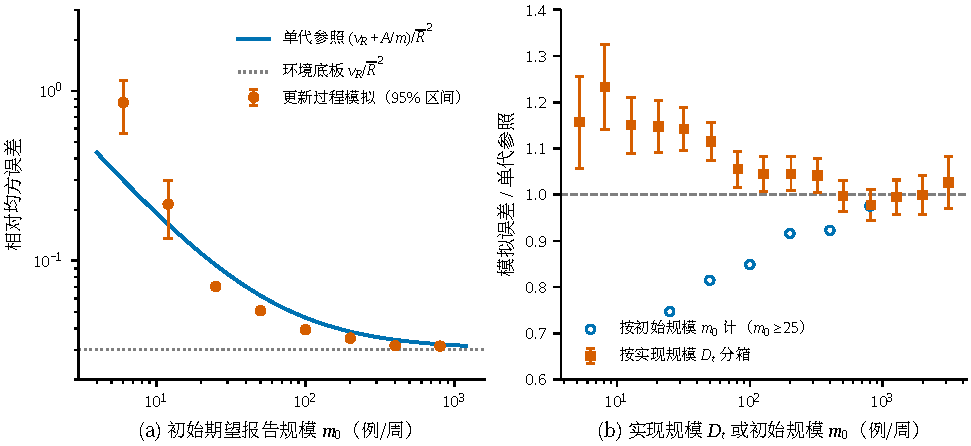
\includegraphics[width=\textwidth]{figures/fig_4_4_renewal_scale.pdf}
  \caption{更新过程仿真中的规模效应。每个初始规模 400 条轨迹，每条 26 个评价点，误差棒为 95\% 区间。（a）增长统计量的相对均方误差随初始规模 $m_0$ 的变化，实线为单代参照曲线 $(v_R+A/m)/\overline{R}^2$，点线为环境底板，参照曲线不是误差下界。（b）模拟误差与参照曲线之比，方块按实际规模 $D_t$ 分组，空心圆按初始规模 $m_0$（$m_0\geq25$）计算。}
  \label{fig:renewal}
\end{figure}

右图把误差与参照曲线之比按两种规模口径分别画出，两种口径给出相反的结论。按初始规模 $m_0$ 计，$m_0\geq25$ 时模拟误差是参照曲线的 0.75--0.98 倍，低于参照。原因是 $\Rbar>1$，疫情在评价期内增长，实际规模高于初始规模，$D_t/m_0$ 的中位数为 1.86--2.35；用初始规模作横轴，等于把较大规模的误差记在了较小规模名下。

按实际规模 $D_t$ 分组，结论反过来。$D_t<400$ 时模拟误差是参照的 1.04--1.23 倍，高于参照，多出的部分来自随机分母：$D_t$ 偶然偏小时，$G_t$ 的分母被低估，比值被放大，而 $1/D_t$ 是凸函数，分母的对称噪声会抬高平均误差。$D_t\geq400$ 时比值为 0.98--1.03，两者基本重合，此时 $D_t$ 中的报告噪声相对很小，随机分母问题消失。

$m_0$ 很小时误差分布有重尾。$m_0=12$ 时比值为 1.31；$m_0=6$ 时为 2.87，且标准误很大，这一数值不稳定。小规模时偶尔出现的近零分母会产生极大的比值，少数几个极端值就能主导均方误差。

由此可以得到两点结论。第一点关于口径：参照曲线是高估还是低估误差，取决于横轴用哪种规模。按实际规模计，“常数加规模反比”的形状大体成立，小规模处误差略高，这为第五章用 $a+b/D_t$ 拟合实证误差提供了依据，也提示第五章的横轴应取实际规模 $D_t$。第二点关于 H4：仿真中各周 $R_t$ 相互独立，$D_t$ 与当期环境无关，H4 在条件意义上仍然成立。真实数据中 $R_t$ 有时间相关，规模大的时期往往也是 $R$ 偏高的时期，H4 不再成立，这会进一步抬高实证截距与斜率。第五章对截距与斜率的分析将回到这一点。

\section{本章小结}
\label{sec:design-summary}

本章把第三章的方差结构转化为三类监测设计结论，并检验了单代结论在时间序列中的适用程度。总报告量固定时，规模项与切分方式无关，期数越多环境项越小。环境存在一阶自回归相关时，常用的有效期数近似会高估环境项，流感季常见的二三十周、强相关情形下高估可达两成到六成以上。引入每期固定成本后，成本最优单期规模是成本比与交叉点的几何平均，与两阶段抽样的费用最优分配同构。整数约束下的最优方案与连续解相差约 2.5\%，正相关使最优方案偏向更多、更小的期。判断当期增长时，Wald 检验在小规模下超出名义水平，基于负二项分布函数的精确检验可以控制水平；稳定检出 15\% 的增长需要约十倍于示例交叉点的规模。

更新过程仿真表明，真实序列中的分母是随机的，单代公式只能作参照曲线。按实际规模计，误差形状与参照曲线大体一致，小规模处偏高；按初始规模计则偏低。第五章将以实际规模为横轴，在美国流感住院数据上检验“常数加规模反比”的误差形状。
